\chapter{Testování}
\label{chap:testovani}

Testování aplikace kombinuje automatizované testy na úrovni backendu s~manuálním testováním uživatelského rozhraní a~telemetrického systému. Cílem je ověřit správnost klíčových funkcionalit -- autentizace, správy obsahu, náborového procesu a~příjmu telemetrických dat.

\section{Metodika testování}

\subsection{Unit testy}

Unit testy ověřují správnost izolovaných jednotek kódu -- validačních schémat, JWT operací a~pomocných funkcí pro nahrávání souborů. Testy jsou implementovány ve frameworku \textbf{Jest} s~transpilerem \textbf{ts-jest} pro podporu TypeScriptu. Kvůli ESM modulům vyžaduje spuštění příznak \texttt{--experimental-vm-modules}.

Testováno je několik oblastí:

\begin{itemize}
    \item \textbf{JWT knihovna} -- generování tokenu, unikátnost tokenů pro různé uživatele, správnost payloadu (userId, email, role, expirace), ověření platného tokenu, odmítnutí neplatného/expirovaného/podvrženého tokenu.
    \item \textbf{Auth middleware} -- odmítnutí požadavku bez hlavičky, s~chybným formátem, s~neplatným tokenem; přijetí požadavku s~platným tokenem; kontrola role pro administrátorské endpointy.
    \item \textbf{Validační schémata} -- ověření Zod schémat pro všechny entity (články, události, členy, projekty, autentizaci). Testy pokrývají platná data, chybějící povinná pole, neplatné hodnoty výčtových typů a~volitelná pole.
    \item \textbf{Nahrávání souborů} -- validace MIME (Multipurpose Internet Mail Extensions) typů, kontrola velikostních limitů, generování unikátních názvů, práce se souborovým systémem.
\end{itemize}

\subsection{Integrační testy}

Integrační testy ověřují chování API endpointů jako celku -- od přijetí HTTP požadavku přes middleware řetězec, validaci, zpracování business logiky až po vrácení odpovědi. Na rozdíl od unit testů, které testují izolované funkce, integrační testy simulují reálné požadavky prostřednictvím vestavěné metody \texttt{app.request()} frameworku Hono.

Databázová vrstva je nahrazena mock objektem, což umožňuje testovat aplikační logiku bez závislosti na běžící databázi. JWT tokeny jsou generovány skutečnou knihovnou, takže autentizační middleware pracuje autenticky.

Integrační testy pokrývají tři klíčové workflow:

\begin{itemize}
    \item \textbf{Autentizace} -- přihlášení s~platnými i~neplatnými údaji, validace vstupních polí (chybějící e-mail, krátké heslo, neplatný formát).
    \item \textbf{CRUD článků} -- čtení publikovaných článků bez autentizace, čtení všech článků s~autentizací, vytvoření/editace/smazání s~tokenem, odmítnutí bez tokenu (401), vyhledávání podle slugu, 404 pro neexistující záznamy.
    \item \textbf{Náborový proces} -- vytvoření draftu, načtení draftu s~ověřením e-mailu, aktualizace, finalizace (draft $\rightarrow$ pending), odmítnutí opakované finalizace~(409), seznam přihlášek pro administrátora, odmítnutí přístupu bez autentizace. Součástí jsou i~testy konfigurace náboru -- veřejný endpoint pro načtení rolí a~úkolů, administrátorské čtení a~aktualizace nastavení včetně ověření, že veřejný endpoint nevrací interní pole.
\end{itemize}

\subsection{Manuální testování}

Funkcionality, které nelze efektivně pokrýt automatizovanými testy -- zejména uživatelské rozhraní, vizuální správnost a~interakce mezi komponentami -- byly ověřovány manuálně:

\begin{itemize}
    \item \textbf{API} -- testování endpointů přes Swagger UI (\texttt{/docs}), ověření stavových kódů, formátu odpovědí a~chybových hlášení.
    \item \textbf{Administrace} -- průchod CRUD operacemi pro všechny entity, ověření rich-text editoru, nahrávání obrázků, správa knihovny médií.
    \item \textbf{Veřejný web} -- kontrola zobrazení obsahu, responzivního designu na mobilních zařízeních a~funkčnosti navigace.
    \item \textbf{Náborový formulář} -- kompletní průchod všemi šesti kroky, ověření ukládání draftu, pokračování přes e-mailový odkaz, doručení notifikačních e-mailů v~Mail\-Hog.
\end{itemize}

\subsection{Testování telemetrie}

Telemetrický systém je testován prostřednictvím simulátoru popsaného v~kapitole~\ref{chap:implementace}. Simulátor generuje realistická data publikovaná na MQTT broker, čímž umožňuje ověřit celý řetězec od příjmu dat přes Go server až po vizualizaci v~prohlížeči bez nutnosti fyzického raketového startu.

Testovány byly následující scénáře:
\begin{itemize}
    \item Připojení k~live session a~zobrazení dat v~grafech v~reálném čase.
    \item Přepnutí kanálu (A/B/A+B) a~ověření nezávislosti datových toků.
    \item Chování při výpadku dat (blackout) -- detekce, indikátor, prodloužení poslední hodnoty.
    \item Prohlížení historických dat s~různým rozlišením a~export do CSV/JSON.
\end{itemize}

\section{Výsledky testování}

\subsection{Automatizované testy}

Celkem 112~testů v~7~testovacích suitách prochází úspěšně. Tabulka~\ref{tab:test-results} shrnuje výsledky podle kategorií.

\begin{table}[ht]
\centering
\small
\begin{tabular}{llrl}
\hline
\textbf{Kategorie} & \textbf{Suita} & \textbf{Testů} & \textbf{Výsledek} \\
\hline
Unit & Auth middleware & 8 & \textit{pass} \\
Unit & JWT knihovna & 10 & \textit{pass} \\
Unit & Validační schémata (5~entit) & 30 & \textit{pass} \\
Unit & Nahrávání souborů & 16 & \textit{pass} \\
Integrační & Auth endpoint & 7 & \textit{pass} \\
Integrační & Articles CRUD & 15 & \textit{pass} \\
Integrační & Recruitment workflow + settings & 26 & \textit{pass} \\
\hline
\textbf{Celkem} & & \textbf{112} & \textbf{pass} \\
\hline
\end{tabular}
\caption{Výsledky automatizovaných testů.}
\label{tab:test-results}
\end{table}

\subsection{Manuální testovací scénáře}

Manuální testování pokrylo čtyři hlavní oblasti aplikace. V~rámci \textbf{autentizace} bylo ověřeno přihlášení s~platnými i~neplatnými údaji, přesměrování nepřihlášeného uživatele z~administrace na přihlašovací stránku a~naopak přesměrování přihlášeného uživatele z~login stránky na dashboard.

V~oblasti \textbf{správy obsahu} byl testován kompletní CRUD cyklus pro všechny entity -- vytvoření článku s~obrázkem a~rich-text obsahem, editace události se změnou statusu, smazání projektu, správa členů a~partnerů. U~každé operace bylo ověřeno, že se změna projeví jak v~administraci, tak na veřejném webu.

\textbf{Náborový formulář} byl testován průchodem všemi osmi kroky, ověřením automatického ukládání rozpracované přihlášky, pokračováním v~draftu prostřednictvím odkazu zaslaného e-mailem a~doručením potvrzovacích e-mailů v~testovacím prostředí MailHog.

U~\textbf{telemetrického systému} bylo ověřeno připojení k~live session se spuštěným simulátorem, zobrazení dat v~grafech v~reálném čase, prohlížení historických dat s~různým rozlišením a~export dat do formátu CSV. Testováno bylo také chování při výpadku dat -- detekce výpadku, zobrazení varovného indikátoru a~prodloužení poslední známé hodnoty v~grafech.

Všechny testované scénáře proběhly úspěšně včetně ověření responzivního designu na mobilních zařízeních.

\subsection{Porovnání úrovní kvality doručení MQTT}
\label{sec:qos-benchmark}

\begin{sloppypar}
Pro ověření volby QoS~1 pro telemetrická data byl proveden benchmark porovnávající všechny tři úrovně kvality doručení protokolu MQTT (QoS~0, 1 a~2) při pěti reprezentativních frekvencích odesílání zpráv v~rozsahu 10--500\,Hz. Každá konfigurace běžela po~dobu 30~sekund s~payloadem o~velikosti přibližně 1\,KB, odpovídajícím rozšířené telemetrické zprávě (GPS, rychlost, senzory, gyro, stav motoru). Měřena byla průměrná latence, latence 95.~percentilu (P95) a~podíl ztracených zpráv. Benchmark byl spuštěn proti produkčnímu Mosquitto brokeru na~platformě Railway prostřednictvím WebSocket spojení (WSS -- WebSocket Secure).
\end{sloppypar}

Výsledky jsou shrnuty v~tabulce~\ref{tab:qos-remote}. Latence je vizualizována na~obrázku~\ref{fig:qos-latency-combined} a~ztráty zpráv na~obrázku~\ref{fig:qos-loss}.

\begin{table}[ht]
\centering
\small
\begin{tabular}{ccrrrrr}
\hline
\textbf{QoS} & \textbf{Frekvence} & \textbf{Odesláno} & \textbf{Přijato} & \textbf{Ztráty} & \textbf{Avg (ms)} & \textbf{P95 (ms)} \\
\hline
0 & 10\,Hz  & 300   & 300   & 0,0\,\%  & 66    & 221 \\
1 & 10\,Hz  & 300   & 300   & 0,0\,\%  & 64    & 222 \\
2 & 10\,Hz  & 300   & 300   & 0,0\,\%  & 89    & 109 \\
\hline
0 & 50\,Hz  & 1500  & 1500  & 0,0\,\%  & 47    & 62 \\
1 & 50\,Hz  & 1499  & 1499  & 0,0\,\%  & 46    & 64 \\
2 & 50\,Hz  & 1497  & 1497  & 0,0\,\%  & 94    & 118 \\
\hline
0 & 100\,Hz & 2997  & 2997  & 0,0\,\%  & 46    & 62 \\
1 & 100\,Hz & 2981  & 2981  & 0,0\,\%  & 48    & 67 \\
2 & 100\,Hz & 2987  & 2987  & 0,0\,\%  & 94    & 118 \\
\hline
0 & 200\,Hz & 5943  & 5943  & 0,0\,\%  & 48    & 64 \\
1 & 200\,Hz & 5932  & 5932  & 0,0\,\%  & 198   & 761 \\
2 & 200\,Hz & 5975  & 5968  & 0,1\,\%  & 790   & 1212 \\
\hline
0 & 500\,Hz & 14592 & 14592 & 0,0\,\%  & 56    & 82 \\
1 & 500\,Hz & 14828 & 11602 & 21,8\,\% & 2424  & 3233 \\
2 & 500\,Hz & 14820 & 4718  & 68,2\,\% & 5443  & 8484 \\
\hline
\end{tabular}
\caption{Porovnání latence a~ztrát MQTT při různých úrovních QoS -- vzdálený server (Railway, WSS, 30\,s, payload $\sim$1\,KB).}
\label{tab:qos-remote}
\end{table}

\begin{figure}[H]
\centering
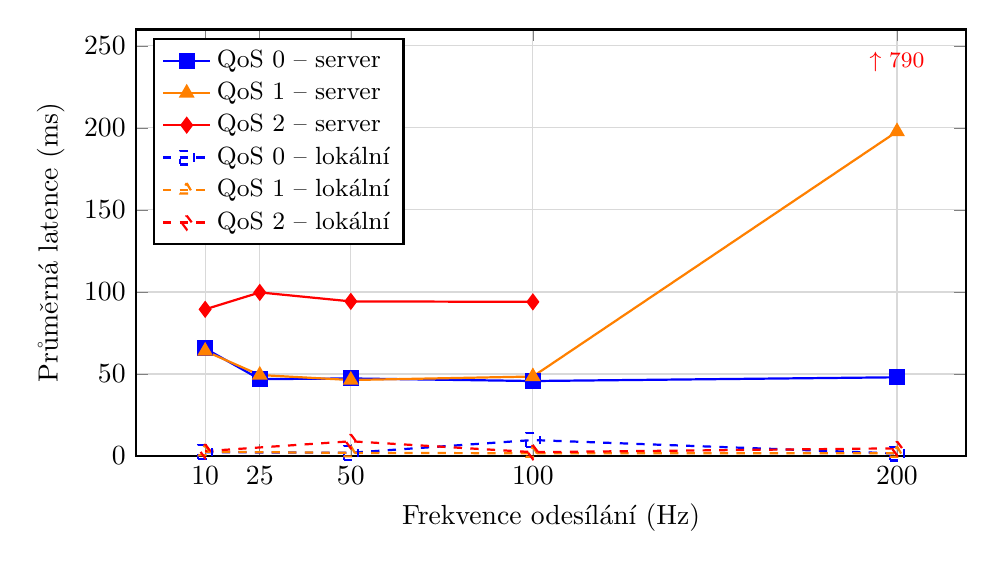
\begin{tikzpicture}
\begin{axis}[
    width=\textwidth,
    height=7cm,
    ylabel={Průměrná latence (ms)},
    xlabel={Frekvence odesílání (Hz)},
    xtick={10, 25, 50, 100, 200},
    ymin=0,
    ymax=260,
    /pgf/number format/use comma,
    legend style={at={(0.02,0.98)}, anchor=north west, font=\small, cells={anchor=west}},
    grid=major,
    grid style={gray!30},
    thick,
    clip=false,
]
% Vzdálený server (plná čára)
\addplot[color=blue, mark=square*, mark size=2.5pt, solid] coordinates {(10, 65.56) (25, 46.86) (50, 47.29) (100, 45.72) (200, 48.00)};
\addplot[color=orange, mark=triangle*, mark size=2.5pt, solid] coordinates {(10, 64.00) (25, 49.38) (50, 46.33) (100, 48.46) (200, 197.76)};
\addplot[color=red, mark=diamond*, mark size=2.5pt, solid] coordinates {(10, 89.41) (25, 99.71) (50, 94.25) (100, 93.96)};
% QoS 2 @ 200 Hz = 790 ms — mimo rozsah, znázorněno šipkou
\node[red, font=\footnotesize] at (axis cs:200, 240) {$\uparrow$ 790};
% Lokální prostředí (čárkovaná)
\addplot[color=blue, mark=square, mark size=2.5pt, dashed] coordinates {(10, 2.33) (50, 1.99) (100, 9.76) (200, 1.53)};
\addplot[color=orange, mark=triangle, mark size=2.5pt, dashed] coordinates {(10, 2.62) (50, 1.92) (100, 1.70) (200, 1.67)};
\addplot[color=red, mark=diamond, mark size=2.5pt, dashed] coordinates {(10, 2.98) (50, 9.00) (100, 2.37) (200, 4.70)};
\legend{QoS 0 -- server, QoS 1 -- server, QoS 2 -- server, QoS 0 -- lokální, QoS 1 -- lokální, QoS 2 -- lokální}
\end{axis}
\end{tikzpicture}
\caption{Průměrná latence MQTT při frekvencích 10--200\,Hz. Plné čáry: vzdálený server (Railway, WSS, 1\,KB payload), čárkované: lokální prostředí. Hodnota QoS~2 při 200\,Hz (790\,ms) přesahuje rozsah grafu a~je zde naznačena šipkou.}
\label{fig:qos-latency-combined}
\end{figure}

\begin{figure}[H]
\centering
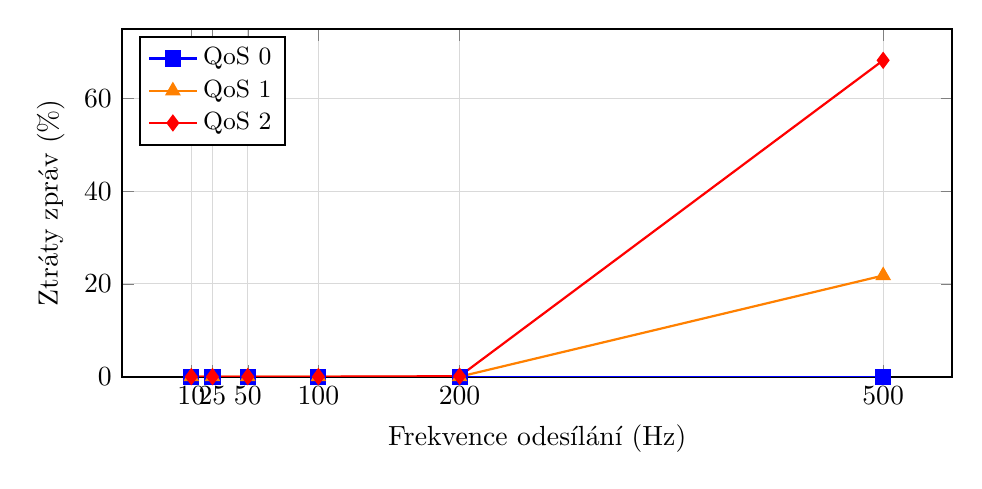
\begin{tikzpicture}
\begin{axis}[
    width=\textwidth,
    height=6cm,
    ylabel={Ztráty zpráv (\%)},
    xlabel={Frekvence odesílání (Hz)},
    xtick={10, 25, 50, 100, 200, 500},
    ymin=0,
    ymax=75,
    /pgf/number format/use comma,
    legend style={at={(0.02,0.98)}, anchor=north west, font=\small, cells={anchor=west}},
    grid=major,
    grid style={gray!30},
    thick,
]
\addplot[color=blue, mark=square*, mark size=2.5pt, solid] coordinates {(10, 0) (25, 0) (50, 0) (100, 0) (200, 0) (500, 0)};
\addplot[color=orange, mark=triangle*, mark size=2.5pt, solid] coordinates {(10, 0) (25, 0) (50, 0) (100, 0) (200, 0) (500, 21.8)};
\addplot[color=red, mark=diamond*, mark size=2.5pt, solid] coordinates {(10, 0) (25, 0) (50, 0) (100, 0) (200, 0.1) (500, 68.2)};
\legend{QoS 0, QoS 1, QoS 2}
\end{axis}
\end{tikzpicture}
\caption{Ztráty zpráv na vzdáleném serveru (Railway, WSS, 1\,KB payload) při rostoucí frekvenci odesílání.}
\label{fig:qos-loss}
\end{figure}

Při frekvencích do~100\,Hz dosahují QoS~0 a~QoS~1 srovnatelné latence (46--66\,ms) bez ztrát. QoS~2 vykazuje přibližně dvojnásobnou latenci (přibližně 90\,ms) vlivem čtyřkrokového handshake (PUBLISH/PUBREC/PUBREL/PUBCOMP). Od~200\,Hz se rozdíly prohlubují -- QoS~1 zpomaluje na~198\,ms a~QoS~2 na~790\,ms s~prvními ztrátami, zatímco QoS~0 zůstává na~stabilních 48\,ms. Při 500\,Hz režie potvrzovacích mechanismů paradoxně způsobuje zahlcení brokeru -- QoS~1 ztrácí 21,8\,\% zpráv a~QoS~2 přes 68\,\%, zatímco QoS~0 doručí všechny zprávy. Ztráty u~QoS~1 a~2 však nepředstavují nevratnou ztrátu dat -- zprávy se hromadí ve~frontě brokeru a~po~ustálení zátěže se zpožděně doručí a~uloží do~InfluxDB.

Výsledky potvrzují vhodnost volby QoS~1 pro telemetrický systém. Při frekvencích typických pro raketovou telemetrii (10--50\,Hz) poskytuje garanci doručení bez dopadu na latenci a~zajišťuje kompletnost dat i~při nestabilním připojení pozemní stanice -- na rozdíl od QoS~0, kde jsou data z~doby výpadku nenávratně ztracena. Úroveň QoS~2 přináší zbytečnou režii, protože případné duplicitní doručení u~QoS~1 nepředstavuje problém -- InfluxDB přepíše datový bod se stejným časovým razítkem.

\section{Identifikované problémy}

V~průběhu testování bylo identifikováno a~opraveno několik problémů.

\subsection{Databázové a validační problémy}

\begin{itemize}
    \item \textbf{VARCHAR overflow} -- náborový formulář generoval delší texty, než povoloval databázový sloupec typu \texttt{VARCHAR}. Řešením byl přechod na typ \texttt{TEXT} pro volné textové vstupy.
    \item \textbf{Duplicitní náborové záznamy} -- při odeslání nové přihlášky se vytvářel nový záznam místo finalizace existujícího draftu. Opraveno úpravou logiky na finalizaci draftu změnou statusu.
    \item \textbf{Dashboard statistiky} -- chybné názvy sloupců v~agregačních dotazech (\texttt{m.active} místo \texttt{m.is\-Active}) a~nesprávný filtr pro aktivní projekty. Opraveno sladěním s~databázovým schématem.
    \item \textbf{Validační schémata v~testech} -- existující testy obsahovaly nesprávné hodnoty statusů a~chybějící povinná pole, které neodpovídaly aktuálním Zod schématům. Opraveno aktualizací testovacích dat.
\end{itemize}

\subsection{Problémy v~modulu článků}

Modul pro správu článků obsahoval problémy, které se projevily až při manuálním testování uživatelského rozhraní. Společným jmenovatelem těchto chyb bylo, že jednotlivé komponenty fungovaly samostatně správně, ale při integraci s~ostatními částmi aplikace způsobovaly neočekávané chování. Tyto problémy vznikaly typicky u~kódu generovaného AI nástroji, kde chyběl kontext o~okolních částech aplikace. Jejich odhalení vyžadovalo ruční průchod celým workflow -- od~vytvoření článku přes přidání obrázků až~po~zobrazení na~veřejném webu.

\begin{itemize}
    \item \textbf{Nechtěné odeslání formuláře při výběru obrázku.} Komponenta pro výběr obrázků z~knihovny médií fungovala správně při izolovaném použití, ale po vložení do formuláře článku způsobovala jeho nechtěné odeslání. Příčinou bylo, že tlačítka neměla nastavený atribut \texttt{type="button"} -- výchozí typ v~HTML formuláři je \texttt{submit}, takže kliknutí na obrázek odeslalo formulář s~neúplnými daty. Opraveno přidáním atributu a~implementací parsování validačních chyb do srozumitelných českých hlášek.

    \item \textbf{Plánované publikování článků.} Původní implementace nezohledňovala datum publikování při zobrazování článků -- článek se statusem \texttt{published} a~budoucím datem byl ihned viditelný na veřejném webu. Přidán filtr na úrovni API, který na veřejných endpointech vrací pouze články s~datem publikování v~minulosti, čímž administrátor může připravit článek dopředu a~nastavit přesný čas zveřejnění.
\end{itemize}

\subsection{Migrace rich-text editoru}
\label{sec:test-richtext}

Původní rich-text editor \texttt{react-quill-new}, zvolený na základě doporučení AI nástroje, generoval nestandardní HTML výstup -- například seznamy bez obalových elementů \texttt{<ul>}/\texttt{<ol>}, místo toho s~vlastními CSS třídami. Obsah se v~editoru zobrazoval správně, ale na veřejném webu byl rozbitý. Na základě tohoto zjištění byla provedena migrace na knihovnu \textbf{Tiptap}, která generuje standardní HTML. Rozhraní komponenty zůstalo zachováno, takže existující obsah v~databázi nevyžadoval úpravy. Implementace editoru je popsána v~sekci~\ref{sec:impl-richtext}.
